\documentclass[14pt]{article}

\usepackage[russian]{babel}
\usepackage[utf8]{inputenc}
\usepackage{amsmath,amssymb}
\usepackage{parskip}
\usepackage{caption}
\usepackage{textcomp}
\usepackage{gensymb}
\usepackage[dvips]{graphicx}
\usepackage{wrapfig}
\usepackage{color}
\usepackage{setspace}
%\usepackage{hyperref}
\usepackage{epstopdf}

\oddsidemargin=0 cm
\evensidemargin=0 cm
\textwidth=170 mm
\textheight=230 mm
\topmargin=0 cm
\voffset= -2cm
\pagenumbering{false}
\newlength{\varheight}
\setlength{\varheight}{3.1cm}
\setlength{\parindent}{0cm}
\spacing{1.1}
\parskip=2mm
\clubpenalty=10000
\widowpenalty=10000
\captionsetup[figure]{labelformat=empty}

\begin{document}

\begin{center}
\Large{\textbf{Комплексные импедансы - 1}}

\textbf{16.04.2017}

\vspace{5mm}
\end{center}

\begin{wrapfigure}{r}{130pt}
\begin{center}
\vspace{-5mm}
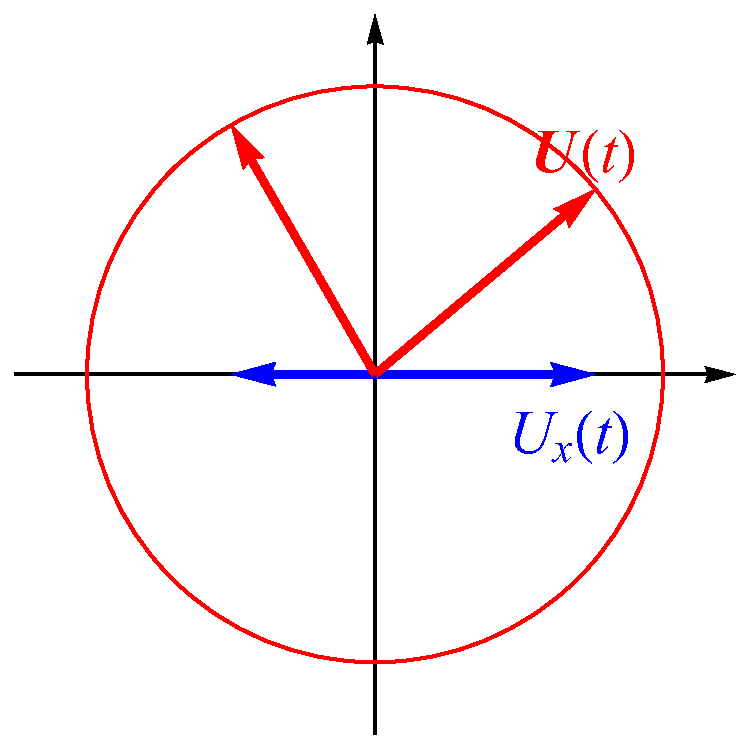
\includegraphics[scale=0.35]{impedance1.pdf}
\caption{\hspace{-2.5mm}К задаче 1}
\end{center}
\vspace{-6mm}
\end{wrapfigure}

Внимание! В данной подборке мнимая единица обозначается буквой $j$ во избежание путаницы с токами $i$.

1. Найдите координаты постоянного по модулю и непрерывного по времени вектора $\vec{U}(t)$ на плоскости $xOy$, проекция которого на ось $Ox$ зависит от времени по закону $U_x(t)=U_0\cos\omega t$ (у данной задачи 2 ответа, выберите вращающийся против часовой стрелки). Параметризуйте плоскость $xOy$ множеством комплексных чисел. Чему равняется соответствующее вектору $\vec{U}(t)$ комплексное число $\tilde{U}(t)$?

2. Пусть ток и напряжение в некоторой схеме изменяются по гармоническому закону с частотой $\omega$. Выберем начало отсчета времени так, чтобы напряжение изменялось по закону $u(t)=u_0\cos\omega t$. При этом ток будет задаваться формулой $i(t)=i_0\cos (\omega t+\varphi)$, где $\varphi$ --- разность фаз между током и напряжением.

а) Найдите постоянные по модулю комплексные величины $\tilde{u}(t)$ и $\tilde{\imath}(t)$ (см. задачу 1), соответствующие величинам $u(t)$ и $i(t)$ (т.е. такие, что $u(t)=\text{Re}\,\tilde{u}(t)$ и $i(t)=\text{Re}\,\tilde{\imath}(t)$).

б) Определите среднюю мощность, потребляемую схемой.

в) Покажите, что предыдущий ответ не изменится, если $\tilde{u}(t)$ и $\tilde{\imath}(t)$ одновременно домножить на $e^{j\theta(t)}$ (поворот на угол $\theta(t)$), где $\theta(t)$ --- произвольная функция времени.

\begin{wrapfigure}{r}{230pt}
\begin{center}
\vspace{-5mm}
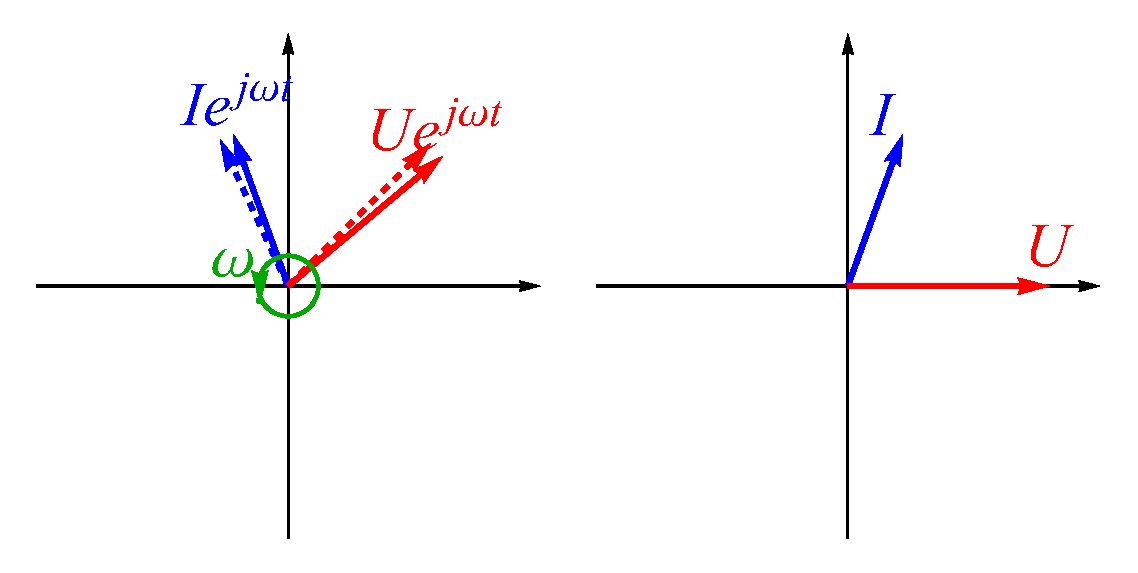
\includegraphics[scale=0.4]{impedance2.pdf}
\end{center}
\vspace{-3mm}
\end{wrapfigure}

Если функции $\tilde{u}(t)$ и $\tilde{\imath}(t)$ брать непосредственно из ответа задачи 2а, то соответствующие им векторы будут вращаться вместе как единое целое с угловой скоростью $\omega$ (рис). Между тем мы выяснили, что домножение на $e^{j\theta(t)}$ не изменяет физику задачи. Поэтому в реальных расчетах схем обычно умножают на $e^{-j\omega t}$, убирая вращение, т.е. фазы всех токов и напряжений отсчитывают от фазы входного напряжения. При этом величины $\tilde{u}$ и $\tilde{\imath}$ на элементах цепи также перестают зависеть от времени (т.к. разность фаз между ними и входным напряжением постоянна и задается лишь параметрами схемы), и их называют соответственно комплексными напряжениями и токами на них. Также, обычно при подсчете комплексных токов и напряжений амплитуду делят на нормировочный множитель $\sqrt2$, чтобы в 2б мощность получалась без численного коэффициента. Таким образом, комплексное напряжение $\tilde{u}(t)=u_0 e^{j\varphi}$ соответствует истинному напряжению $u(t)=u_0\sqrt2 \cos(\omega t+\varphi)$, а $u_0$ называют действущим (эффективным) значением напряжения. Отметим, что по-прежнему домножение комплексных напряжений и токов на $e^{j\delta}$ ничего не изменяет (физически это соответствует изменению фазы на $\delta$, или, что то же самое, сдвижкой по времени на $\delta/\omega$). Далее под напряжением источника переменного тока будем всегда понимать именно действующее значение.

3. Пусть напряжение на резисторе с сопротивлением $R$ изменяется по закону $u(t)$, а ток --- по закону $i(t)$.

а) Найдите связь между этими величинами (закон Ома).

б) Пусть ток в резисторе изменяется по закону $i(t)=i_0\sqrt2 \cos\omega t$. Найдите зависимость напряжения на резисторе $u(t)$ от времени.

в) Найдите соответствующие значения комплексного напряжения и тока $\tilde{u}$ и $\tilde{\imath}$ в резисторе. Покажите, что связь между ними можно записать в виде $\tilde{u}=\tilde{\imath}R$.

4. Пусть напряжение на катушке с индуктивностью $L$ изменяется по закону $u(t)$, а ток --- по закону $i(t)$.

а) Найдите связь между этими величинами.

б) Пусть ток в катушке изменяется по закону $i(t)=i_0\sqrt2 \cos\omega t$. Найдите зависимость напряжения на катушке $u(t)$ от времени.

в) Найдите соответствующие значения комплексного напряжения и тока $\tilde{u}$ и $\tilde{\imath}$ в катушке. Покажите, что связь между ними можно записать в виде $\tilde{u}=\tilde{\imath}X_L$. Найдите $X_L$.

5. Пусть напряжение на конденсаторе с емкостью $C$ изменяется по закону $u(t)$, а ток --- по закону $i(t)$.

а) Найдите связь между этими величинами.

б) Пусть напряжение на конденсаторе изменяется по закону $u(t)=u_0\sqrt2 \cos\omega t$. Найдите зависимость тока через конденсатор $i(t)$ от времени.

в) Найдите соответствующие значения комплексного напряжения и тока $\tilde{u}$ и $\tilde{\imath}$ в конденсаторе. Покажите, что связь между ними можно записать в виде $\tilde{u}=\tilde{\imath}X_C$. Найдите $X_C$.

Таким образом, мы получили, что у конденсаторов и катушек комплексные напряжения и токи связаны таким же соотношением, как и у резистора. Роль сопротивления играют величины $X_L$ и $X_C$ --- их называют комплексными импедансами. Таким образом, для конденсаторов и катушек можно записывать обычный закон Ома, если в качестве напряжений и токов брать комплексные величины. Так, при последовательном включении катушки и конденсатора суммарный импеданс $Z=X_L+X_C$, а при параллельном включении конденсатора и резистора $1/Z=1/R+1/X_C$. Такой метод расчета называется методом комплексных импедансов, и он резко упрощает вычисления, связанные с цепями переменного тока.

6. Подключим последовательно резистор $R$, конденсатор $C$ и катушку $L$ к источнику переменного тока с действующим напряжением $U_0$. Найдите при помощи метода комплексных импедансов действующие напряжения и силы тока элементов цепи, а также их среднюю мощность.

\end{document} 